%%%%%%%%%%%%%%%%%%%%%%%%%%%%%%%%%%%%%%%%%%%%%%%%%%%%%%%%%%%%%%%%%%%%%%%%%%%%%%%%
%2345678901234567890123456789012345678901234567890123456789012345678901234567890
%        1         2         3         4         5         6         7         8

%\documentclass[letterpaper, 10 pt, conference]{orbieeeconfpre}  % Comment this line out if you need a4paper

\documentclass[a4paper, 10pt, journal]{wissarbIEEE}      % Use this line for a4 paper
%\conference{IEEE Conference for Awesome ORB Research}

\bibliographystyle{orbref-num}


\IEEEoverridecommandlockouts                              % This command is only needed if 
                                                          % you want to use the \thanks command

\overrideIEEEmargins                                      % Needed to meet printer requirements.

% See the \addtolength command later in the file to balance the column lengths
% on the last page of the document

\usepackage{hyperref}
\usepackage{graphicx}
\usepackage{tabularx}
\usepackage{booktabs}
\usepackage{lipsum}

\title{\LARGE \bf
The crowd congestion level - a new measure for risk assessment in video-based crowd monitoring
}

\author{Sebastian Bek$^{1}$ and Dr.-Ing. Eduardo Monari$^{2}$% <-this % stops a space
\thanks{*Based on the guidelines published on the \href{http://conf.papercept.net/conferences/support/tex.php}{PaperCept conference manuscript management website}}% <-this % stops a space
\thanks{$^{1}$Sebastian Bek is with the master program for Applied Computer Science at the Institute for Computer Science, Heidelberg University
        {\tt\small sebibek@gmail.com}}%
\thanks{$^{2}$Dr.-Ing. Eduardo Monari, is with the Department of Video Exploitation Systems (VID), Fraunhofer Institute for Optronics System Technology and Image Exploitation (IOSB), Fraunhoferstraße 1, 76131 Karlsruhe
        {\tt\small eduardo.monari@iosb.fraunhofer.de, \href{https://www.iosb.fraunhofer.de}{}}}%
}


\begin{document}



\maketitle

%%%%%%%%%%%%%%%%%%%%%%%%%%%%%%%%%%%%%%%%%%%%%%%%%%%%%%%%%%%%%%%%%%%%%%%%%%%%%%%%
\begin{abstract}

In this paper, we propose a new characteristic measure relative crowd density and motion dynamics for the purpose of long-term crowd monitoring. Furthermore, we will discuss the derivation of a so-called Congestion Level of local areas in the crowd, which takes the current dynamics and density within a certain image region into account.

\end{abstract}

%%%%%%%%%%%%%%%%%%%%%%%%%%%%%%%%%%%%%%%%%%%%%%%%%%%%%%%%%%%%%%%%%%%%%%%%%%%%%%%%
\section{Introduction}
\label{sec:intro}
The visitor rates at public events are increasing steadily since several years. In particular, besides large events in closed-area environments (e.g. stadiums, festival areas, etc.) crowds have also become a common phenomenon in public urban environment. In such environments video-based monitoring might be useful for both, safety-related and security-related applications.

\section{State-of-the-art approaches}
\label{sec:sota}
For automated counting of people in images, there exist two main approaches, the so-called direct, and the indirect approach. In direct approaches people are first detected, segmented from background and then counted. Examples for direct approaches can be found in e.g. \cite{rittscher}. The indirect approach however, is considered to be more robustly, since the individual segmentation of persons as foreground regions is itself a challenging problem, that is not solved reliably yet. Yet a promising approach has been proposed by Albiol et al. \cite{albiol}, whereas the number of moving corner features is used to estimate the number of persons in the image region.

\section{Proposed Method}
\label{sec:method}
Since the estimation of dynamics is useful for indication of congestion and flow jams in a crowd, it would be interesting to gather information about them as well. In our approach we use motion (tracks) in the scene as basic features, as well as relative changes in track velocities (inertia) for generation of a so-called Congestion Level. We observed that even in scenarios with high people density, the situation can be regarded as non-critical, in case people can still move freely and smoothly through the crowd. As a consequence, we believe that information on the flow dynamics should be taken into account for risk assessment. Our approach assumes, that a local spot in the crowd might be critical, if the density is continuously increasing (relative density) over time, and simultaneously a significant reduction of motion dynamics (increasing inertia) is observed. The proposed approach is an indirect one, since it is considered to be more robust in case of small objects in the scene. The approach used is similar to the one proposed by Albiol at Al. in \cite{albiol}. However, in addition to just clustering and counting moving features (people counting), we extend the motion vector extraction by multi-frame feature tracking and by estimation of densities and dynamics. The approach used to obtain trajectories from motion features is as follows: (1) Detection of a set of Harris Corners \cite{harris} as pixel coordinates $\mathcal{F} = \{\mathbf{f}_1, \mathbf{f}_2, ..., \mathbf{f}_n\}$, (2) estimation of LK optical flow \cite{LK} for detected features and assignment of resulting motion vectors $\mathcal{V} = \{\mathbf{v}_1, \mathbf{v}_2, ..., \mathbf{v}_n\}$ to each feature, and (3) classification of features/motion vectors above a minimum motion threshold β as moving features:

%% Figure
\begin{figure}[h]
   \centering
   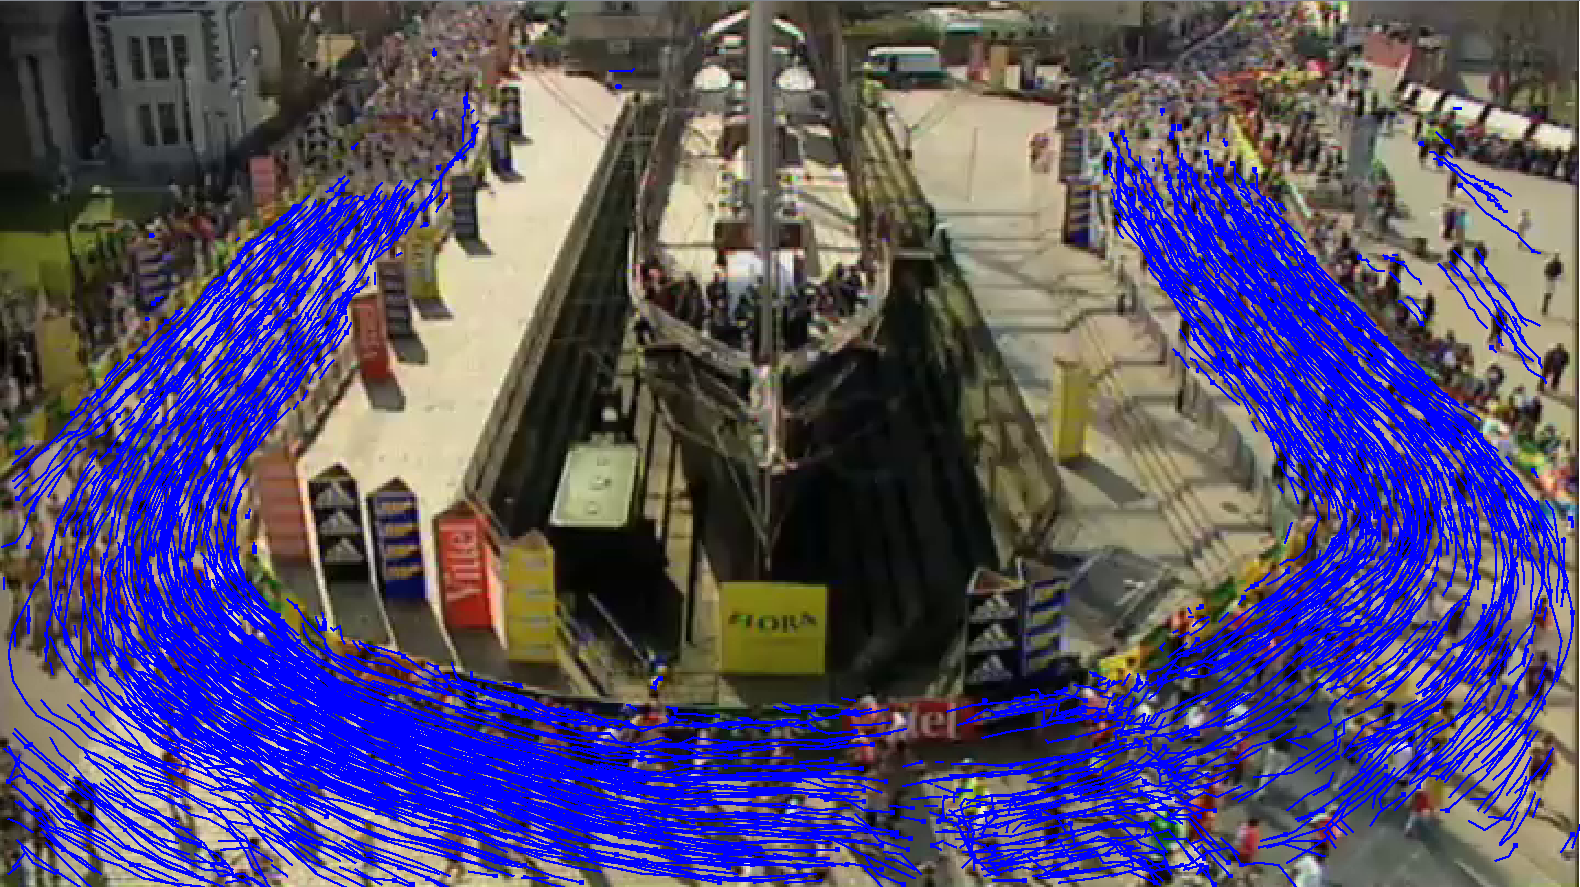
\includegraphics[width=0.35\textwidth]{fig/trajektorien.png}
   \caption{Acquisition of Trajectories (tracklets).}
   \label{fig:trajectories}
\end{figure}

\begin{equation}
	\mathcal{F'} = \{f_i\in \mathcal{F} | \ |v_i| \ge \beta\} \hskip 5pt {with} \ i = \{1..n\}
\end{equation}

Here $f_i=(x,y)^T$ is a feature point located at pixel position $(x,y)$ while $v_i=(\Delta x,\Delta y)$ is the corresponding motion vector, indicating the absolute movement of the feature between the preceding and the current frame. Finally in step (4) motion feature tracking is performed by association of detected moving features to trajectory candidates. In most scenes, this simple classification will sort out almost any detected feature point not corresponding to a moving object (e.g. person). Additionally to obtain information about dynamics and flow, the feature points are used to generate tracks, by concatenation of motion vectors. Hereby, we first try to extend previously created trajectories evaluating the distance between new detected features in the last video frame, and the estimated position of features in the previous video frames, shifted by the optical flow motion vector, which is basically a motion prediction. If no previously created trajectories are found in a defined neighborhood, a new trajectory with the corresponding motion vector is created. Finally, we obtain a set of tracks $\mathcal{T}^k = \{\mathcal{T}_1^k, \mathcal{T}_2^k, ..., \mathcal{T}_m^k\}$, summarizing all available $m = |\mathcal{F'}|$ tracks at time $k$. Each track in turn is basically a set of features $\mathcal{T}_j^k = \{ \mathbf{f}^k, \mathbf{f}^{k-1}, ..., \mathbf{f}^{k-s_j}\}, j\in\{1, ..., m\}$, and $s_j$ the length of the track $j$. 
 The trajectories are assigned with IDs for proper identification and managed in a track list. Fig. \ref{fig:trajectories} shows example results of our local feature tracking approach. Now, since we have track information available, we use them to create statistics on track density, dynamics and flow behavior. To generate local, statistics, the image is split into $R$ smaller image patches $\mathcal{P}$ first, whereas $\mathcal{P}_r, r = \{1, ..., R\}$ represents the set of pixels of each patch. The number of estimated persons (local density) is defined as the amount of trajectory (tracklet) tips in a set of feature points $\mathcal{G}_r$ within a patch $\mathcal{P}_r$ in the very last video frame:

\begin{equation}
	d_r = \kappa\cdot|\mathcal{G}_r| \ \ \ \ \ \ \ \ \ [\frac{tracklets}{patch}]
\end{equation}
with $\mathcal{G}_r \supseteq \mathcal{F′}\cap \mathcal{P}_r$.\\

Here $\kappa$ is some heuristically defined scale factor, indicating that the number of feature points (tracklets) can differ from the actual number of persons. 

To efficiently sense dynamics as well, we propose a hypothesis about congestions: \emph{Congestions can be interpreted as a discontinuity in track flow, which equals low excentric dynamics.} Accordingly, we want to measure the excentric dynamics of a track. Therefore, we measure the Euclidean length of each track position vector within the last q frames. This length is then averaged over all tracklets within an image patch. We call this measure local flow inertia:

\begin{equation}
	i_r^k = \frac{1}{|\mathcal{G}_r'|}\sum_{\forall f\in\mathcal{G}_r'} ||f^k, f^{k-q}||_2 \ \ \ \ \ \ \ \ \ [\frac{{px}}{q\cdot {frame}}] 
\end{equation}

with $\mathcal{G}_r′ = \{T\in\mathcal{G}_r | \ |T| \ge q\}$.\\

For higher robustness of the approach, only tracks with a minimum length of q are taken into account. These tracks are summarized by $\mathcal{G}_r′$, as a subset of $\mathcal{G}_r$.

To measure the risk level for the people in the crowd, we propose a combined coefficient, we call congestion level (${cl}$), which incorporates the estimated inertia and dynamics in form of relative (${rel}$) estimates. To generate relative estimates, it is required to set proper thresholds, obtained by theoretical or experimental analysis. Our derived congestion level is defined as the product of the previously decribed characteristic figures $i_{rel}$ and $d_{rel}$:

\begin{equation}
	{cl} = d_{rel}\cdot i_{rel} \ \ \ \ \ \ \ \ \ [\%] 
\end{equation} 

\section{Evaluation}
\label{sec:eval}

To demonstrate the plausibility of the derived measures, we first compared the obtained track density with manually generated ground truth data. Second, we evaluate the difference between the proposed congestion level and the popular density metric. We used both artificial and real video data publicly available. In the following table we compare the estimated density with manually generated ground-truth data in a certain image patch. Also, we show the impact of the included dynamics measure in the derived congestion level. All measures have been averaged by a temporal mean filter over $10$ frames:

%% Table
\begin{table}[h]
%\tiny
\centering
\caption{Evaluation of Estimates (averaged over $10$ frames).}
   \begin{tabularx}{0.5\textwidth}{p{0.03\textwidth}p{0.02\textwidth}p{0.02\textwidth}p{0.02\textwidth}p{0.02\textwidth}p{0.02\textwidth}p{0.02\textwidth}p{0.02\textwidth}p{0.02\textwidth}p{0.02\textwidth}p{0.02\textwidth}}
   		 \toprule 
   		 fr. & $10$ & $20$ & $30$ & $40$ & $50$ & $60$ & $70$ & $80$ & $90$ & $100$ \\
   		 \midrule
		 GT. & $0.34$ & $0.37$ & $0.39$ & $0.46$ & $0.53$ & $0.62$ & $0.67$ & $0.81$ & $0.89$ & $0.95$ \\
		 \midrule
		 rD. & $0.35$ & $0.45$ & $0.49$ & $0.54$ & $0.59$ & $0.65$ & $0.72$ & $0.81$ & $0.88$ & $0.93$ \\
		 \midrule
		 cl. & $0.35$ & $0.07$ & $0.09$ & $0.01$ & $0.19$ & $0.34$ & $0.49$ & $0.81$ & $0.88$ & $0.93$ \\ 
		 \midrule
   \end{tabularx}  \label{tab:eval}
   \vskip 1pt
   \begin{tiny}
	\textbf{index:} \hskip 5pt fr.: frame; \hskip 5pt GT.: ground-truth relative density; \hskip 5pt rD.: relative density; \hskip 5pt cl: congestion level;
	\end{tiny}
\end{table}
It can be observed, that the estimated relative density follows the ground-truth density and is therefore a reasonable measure for risk assessment. Additionally, dynamics are taken into account with the congestion level. The congestion level rises with a little delay, which represents the growing process of congestions/jams. At first, people are congested from high densities. As a consequence, dynamics decrease rapidly. Thus, the congestion level increases a little delayed because the congestions themselves need high densities as a condition to evolve over time.

\section{Conclusion}
\label{sec:conclusion}
In this paper, we proposed a new characteristic measure for density-related risk assessment in crowd analysis, we call 
Congestion Level. This measure indicates the endangering of local areas in a crowd, due to increasing people density by simultaneous reduction of motion dynamics (stop-and- go or slackening of crowd motion). It has been shown that the proposed Congestion Level provides a suitable measure for dynamics and density, which might be of interest for
(semi-)automated risk assessment systems. Future works might include evaluation of applicability for risk assessment in practice.

\bibliography{mybibfile}

\end{document}
